%%%%%%%%%%%%%%%%%%%%%%%%%%%%%%%%%%%%%%%%%%%%%%%%%%%%%%%%%%%%%%%
%
% Welcome to Overleaf --- just edit your LaTeX on the left,
% and we'll compile it for you on the right. If you open the
% 'Share' menu, you can invite other users to edit at the same
% time. See www.overleaf.com/learn for more info. Enjoy!
%
% Note: you can export the pdf to see the result at full
% resolution.
%
%%%%%%%%%%%%%%%%%%%%%%%%%%%%%%%%%%%%%%%%%%%%%%%%%%%%%%%%%%%%%%%
% Intersection of
% Author: Rasmus Pank Roulund
\documentclass{minimal}
\usepackage{tikz}
\usepackage{verbatim}

\begin{comment}
:Title: Intersection of
:Tags: Coordinate systems


This example shows how the ``intersection of`` mechanism of Tikz work. Notice how a horizontal 
line is made from point B to allow the calculation to be done.

Caption: In a fixed exchange regime it might not be possible to reach internal balance 
(full employment and price stability) and external balance (some given level of net export) 
using only fiscal policy. At point B only point C and D can be reached via fiscal policy. 
Only by devaluing the country is able to reach the optimum level at point A.

:Author: Rasmus Pank Roulund

\end{comment}
\usetikzlibrary{arrows}
\begin{document}
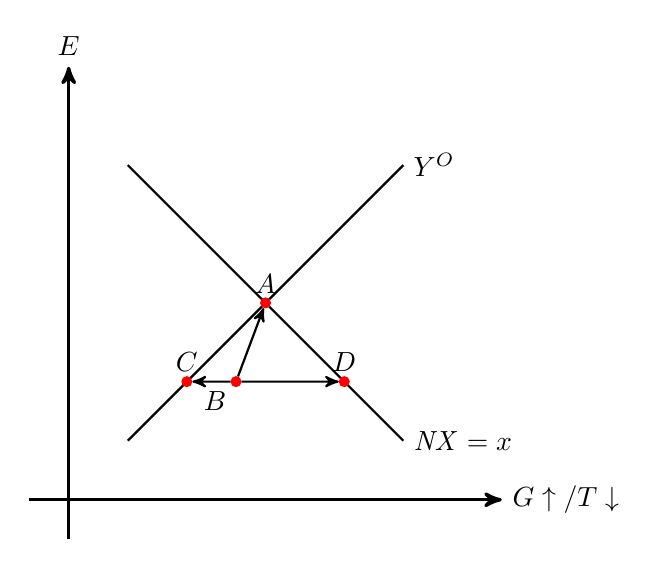
\begin{tikzpicture}[
    scale=5,
    axis/.style={very thick, ->, >=stealth'},
    important line/.style={thick},
    dashed line/.style={dashed, thin},
    pile/.style={thick, ->, >=stealth', shorten <=2pt, shorten
    >=2pt},
    every node/.style={color=black}
    ]
    % axis
    \draw[axis] (-0.1,0)  -- (1.1,0) node(xline)[right]
        {$G\uparrow/T\downarrow$};
    \draw[axis] (0,-0.1) -- (0,1.1) node(yline)[above] {$E$};
    % Lines
    \draw[important line] (.15,.15) coordinate (A) -- (.85,.85)
        coordinate (B) node[right, text width=5em] {$Y^O$};
    \draw[important line] (.15,.85) coordinate (C) -- (.85,.15)
        coordinate (D) node[right, text width=5em] {$\mathit{NX}=x$};
    % Intersection of lines
    \fill[red] (intersection cs:
       first line={(A) -- (B)},
       second line={(C) -- (D)}) coordinate (E) circle (.4pt)
       node[above,] {$A$};
    % The E point is placed more or less randomly
    \fill[red]  (E) +(-.075cm,-.2cm) coordinate (out) circle (.4pt)
        node[below left] {$B$};
    % Line connecting out and ext balances
    \draw [pile] (out) -- (intersection of A--B and out--[shift={(0:1pt)}]out)
        coordinate (extbal);
    \fill[red] (extbal) circle (.4pt) node[above] {$C$};
    % line connecting  out and int balances
    \draw [pile] (out) -- (intersection of C--D and out--[shift={(0:1pt)}]out)
        coordinate (intbal);
    \fill[red] (intbal) circle (.4pt) node[above] {$D$};
    % line between out og all balanced out :)
    \draw[pile] (out) -- (E);
\end{tikzpicture}
\end{document}
%%% Local Variables:
%%% mode: latex
%%% TeX-master: t
%%% End: